\chapter{Dataset Understanding and EDA}\label{chap:eda}

% Helper: wrapped columns for neat 3-col tables
\newcolumntype{P}[1]{>{\raggedright\arraybackslash}p{#1}}

%% ================================================================
%%  PART I — MIMIC-IV for ICD Coding (Problem 1)  [from Old Report]
%% ================================================================
\section{Part I: MIMIC-IV for ICD Coding (Problem 1)}\label{sec:p1:dataset}

\subsection{Overview of MIMIC-IV}\label{sec:p1:mimic_overview}
\noindent
MIMIC-IV is a large, openly accessible database of de-identified electronic health records (EHR), developed through a collaboration between the Beth Israel Deaconess Medical Center (BIDMC) and the Massachusetts Institute of Technology (MIT). It spans clinical encounters from 2008 to 2019 and contains comprehensive data, including demographic information, laboratory values, prescriptions, billing codes, clinical notes, and more. The dataset is organized into multiple modules to reflect different sources or systems:
\begin{itemize}
    \item \texttt{hosp}: Hospital-wide data, containing tables such as \texttt{admissions}, \texttt{patients}, and \texttt{diagnoses\_icd}.
    \item \texttt{icu}: Intensive Care Unit (ICU) data with highly granular time-series measurements (e.g., \texttt{chartevents}).
    \item \texttt{ed}: Emergency department records.
    \item \texttt{note}: De-identified clinical notes, such as discharge summaries.
    \item \texttt{cxr}: Information linking chest X-ray images to the relevant patients in MIMIC-CXR.
\end{itemize}

\vspace{5pt}
\noindent
For the purpose of analyzing discharge summaries and automatically assigning ICD codes, particular emphasis is placed on:
\begin{itemize}
    \item \texttt{patients} in the \textit{hosp} module, which provides demographics such as \texttt{anchor\_age} and \texttt{anchor\_year\_group}.
    \item \texttt{admissions} in the \textit{hosp} module, which contains \texttt{hadm\_id} (hospital admission ID) and timestamps (\texttt{admittime}, \texttt{dischtime}).
    \item \texttt{diagnoses\_icd} in the \textit{hosp} module, indicating both ICD-9 and ICD-10 billed diagnoses.
    \item \texttt{discharge} in the \textit{note} module, offering the textual discharge summaries that are crucial for modeling.
\end{itemize}

\vspace{5pt}
\noindent
All queries used to gather counts, distributions, and other information about the MIMIC-IV dataset were executed via SQL against the MIMIC-IV PostgreSQL database. In the following sections, key outcomes from these queries are summarized, and visual explorations are presented.

\subsection{SQL Query Results and Data Highlights}\label{sec:p1:sql_results}

\subsubsection{Patient and Admission Volumes}
\noindent
SQL queries against the \texttt{patients} and \texttt{admissions} tables determined that there are \textbf{364,627 unique patients} in the \texttt{patients} table. In the \texttt{admissions} table, there are \textbf{546,028 unique admissions}. 

\subsubsection{Multiple Admissions per Patient}
\noindent
An examination of how many admissions each patient has revealed that some patients experience over 100 admissions, highlighting that MIMIC-IV can capture highly recurrent hospital visits for certain individuals.

\subsubsection{Discharge Summaries}
\noindent
Querying the \texttt{discharge} table revealed \textbf{331,793} discharge summaries. Nearly 214,296 admissions in MIMIC-IV do not have a final discharge note, underscoring that not every hospital stay yields a lengthy textual record.

\subsubsection{Characterizing Note Length}
\noindent
Word-count statistics computed for discharge summaries showed that the median note length is approximately 1{,}556 words, and at the 99th percentile, notes can exceed about 3{,}986 words. This wide variation in length indicates that some admissions have minimal documentation, whereas others include very detailed records.

\subsubsection{ICD-9 vs. ICD-10 Utilization}
\noindent
MIMIC-IV contains approximately 3.46 million ICD-10 code assignments and 2.91 million ICD-9 code assignments. This distribution suggests that modern coding practices (ICD-10) have become more prevalent. Detailed counts of top ICD-10 codes revealed chronic conditions like hyperlipidemia (\texttt{E785}) and hypertension (\texttt{I10}) as highly common.

\subsubsection{Long-Tailed Code Distribution}
\noindent
There are \textbf{19,440 unique ICD-10 codes} in the dataset. Around 9,217 ICD-10 codes appear fewer than five times, illustrating the classic long-tail distribution. Models must be robust to rare code occurrences.

\subsubsection{Codes Per Admission}
\noindent
On average, there are \(\sim13.6\) ICD-10 codes billed per admission. Consequently, this setting represents a multi-label classification task: each discharge summary can be associated with numerous codes rather than a single label.

\subsection{Visual Explorations of MIMIC-IV}\label{sec:p1:visual_explorations}

\subsubsection*{Plot 1: Distribution of Anchor Age}
\begin{figure}[H]
    \centering
    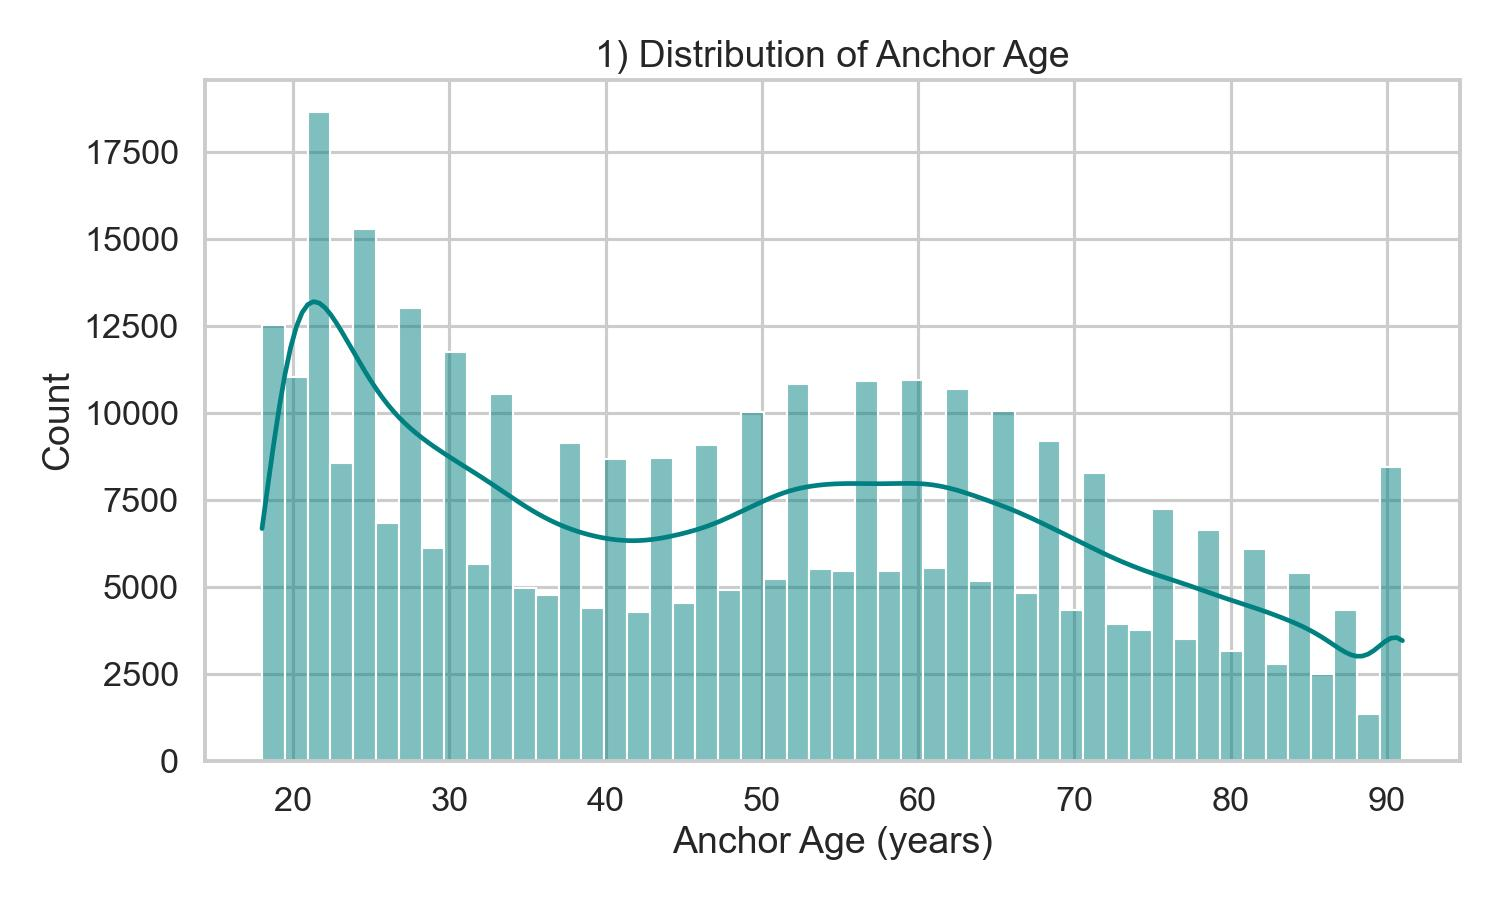
\includegraphics[width=0.5\textwidth]{mimic_plots/plot1.jpg}
    \caption{A histogram revealing a right-skewed distribution of anchor ages, with many individuals in their 20s and 30s.}
    \label{fig:p1:plot1}
\end{figure}

\noindent
Figure~\ref{fig:p1:plot1} shows how anchor ages are concentrated in younger to middle-aged adults, with a tail that extends to the maximum capped age of 91. There is a gradual decrease in frequency after middle age, but a mild uptick near 90--91, reflecting censoring of ages above 89.

\newpage

\subsubsection*{Plot 2: Boxplot of Anchor Age by Admission Type}
\begin{figure}[H]
    \centering
    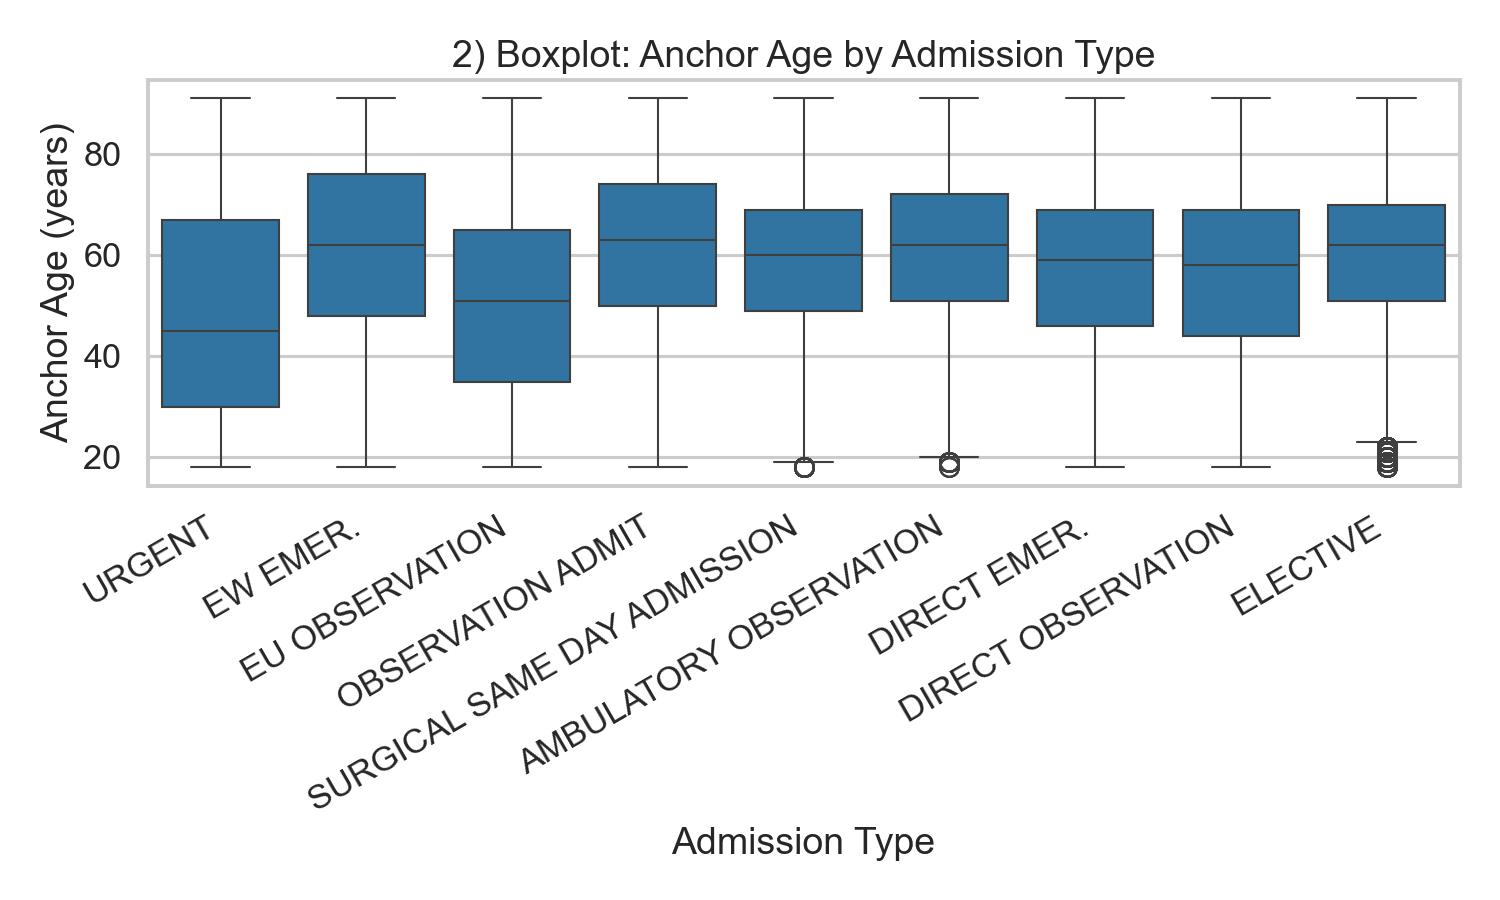
\includegraphics[width=0.5\textwidth]{mimic_plots/plot2.jpg}
    \caption{A boxplot illustrating how anchor age varies across different admission types.}
    \label{fig:p1:plot2}
\end{figure}

\noindent
Figure~\ref{fig:p1:plot2} offers insight into differences in age distributions for various hospital admission pathways (e.g., emergency admissions vs. elective surgeries). Some admission types span a broader age range, while others are more narrowly distributed, reflecting the patient populations associated with particular clinical services.

\newpage

\subsubsection*{Plot 3: Admissions by Anchor Year Group}
\begin{figure}[H]
    \centering
    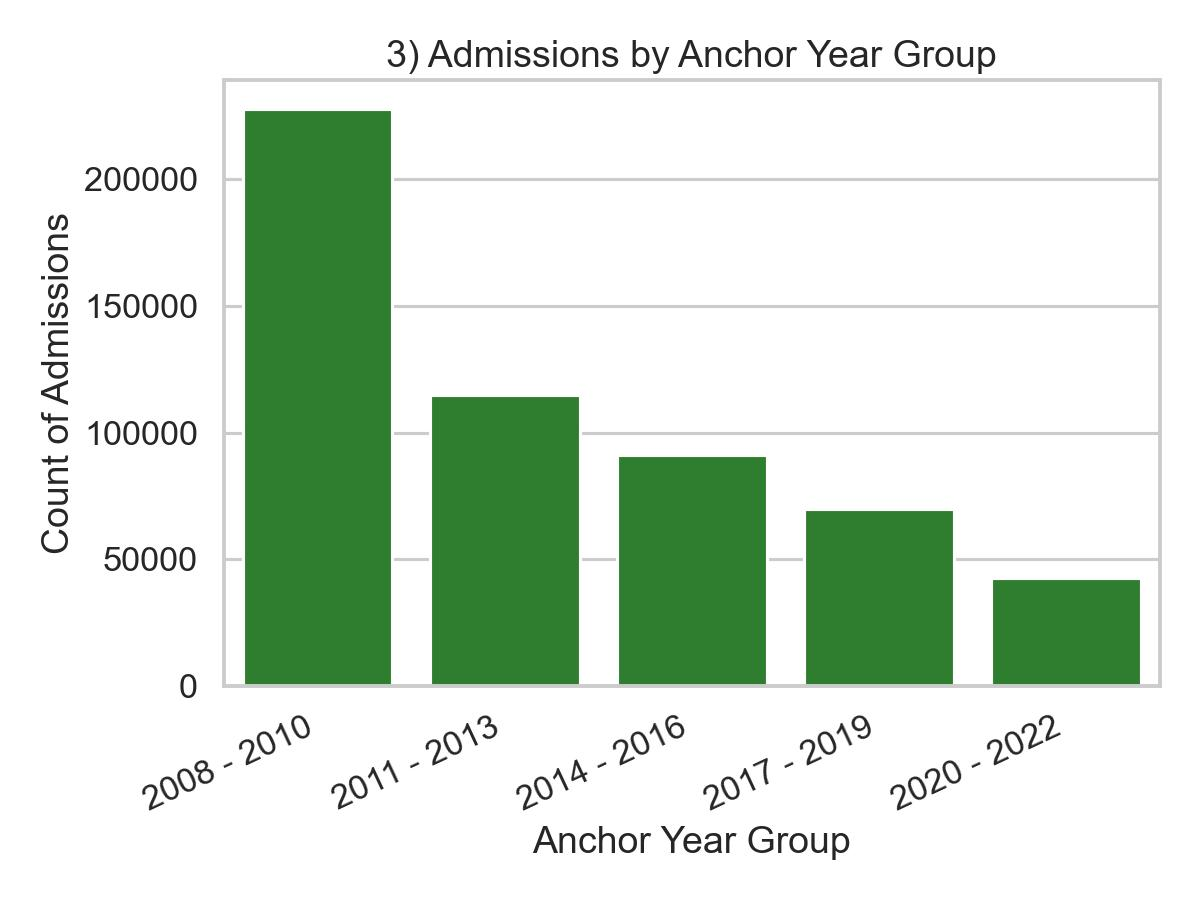
\includegraphics[width=0.5\textwidth]{mimic_plots/plot3.jpg}
    \caption{A bar chart showing the number of admissions categorized by approximate calendar year groups.}
    \label{fig:p1:plot3}
\end{figure}

\noindent
Figure~\ref{fig:p1:plot3} demonstrates a higher number of admissions in the earlier year intervals (2008--2010, 2011--2013) relative to later groups, likely reflecting the data collection periods and any changes in hospital practices over time.

\newpage

\subsubsection*{Plot 4: Top 15 ICD-10 Codes by Frequency}
\begin{figure}[H]
    \centering
    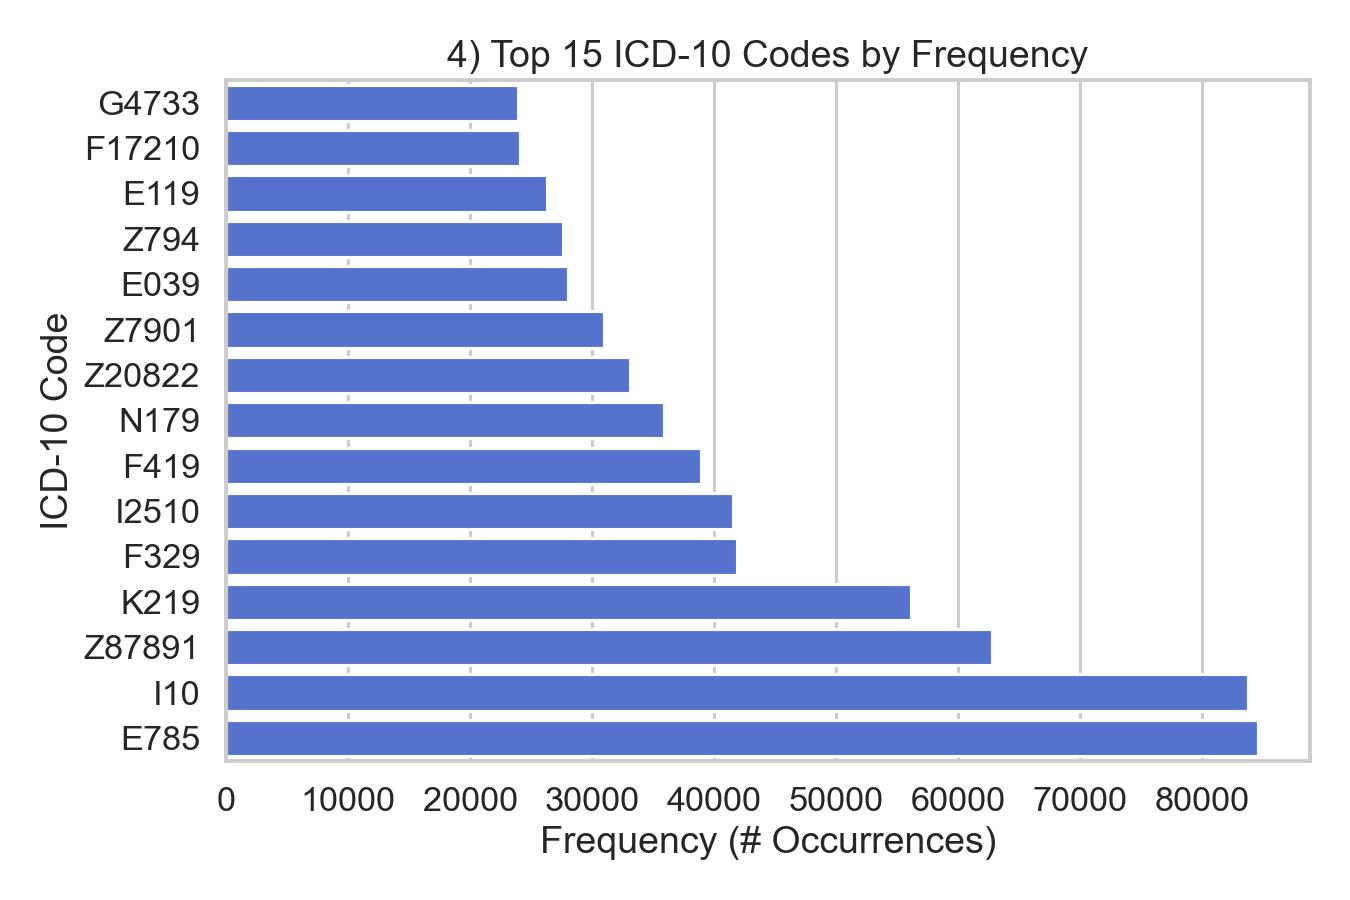
\includegraphics[width=0.5\textwidth]{mimic_plots/plot4.jpg}
    \caption{A horizontal bar chart showing the most common ICD-10 codes among admissions.}
    \label{fig:p1:plot4}
\end{figure}

\noindent
In Figure~\ref{fig:p1:plot4}, chronic conditions such as hyperlipidemia (\texttt{E785}) and hypertension (\texttt{I10}) are clearly visible at the top of the frequency distribution, demonstrating the widespread prevalence of these diagnoses.

\newpage

\subsubsection*{Plot 5: Co-Occurrence Matrix of Top 15 ICD-10 Codes}
\begin{figure}[H]
    \centering
    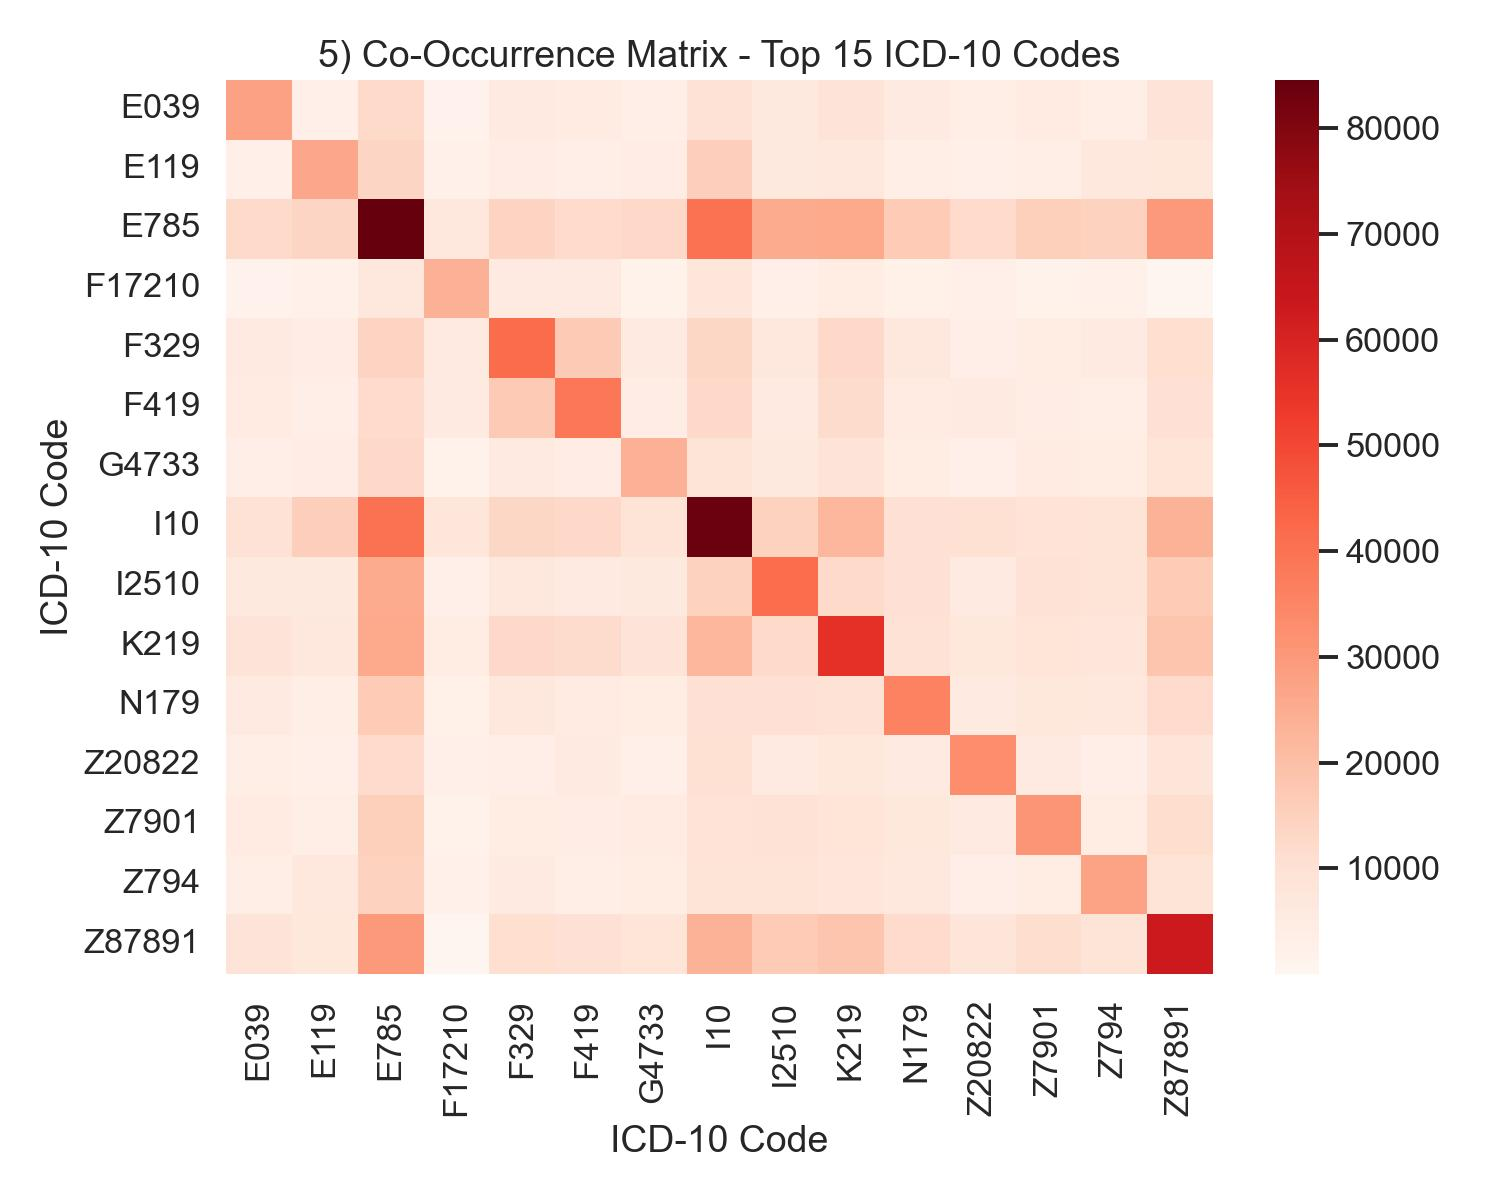
\includegraphics[width=0.5\textwidth]{mimic_plots/plot5.jpg}
    \caption{A heatmap illustrating how frequently pairs of the top 15 ICD-10 codes co-occur within the same admission.}
    \label{fig:p1:plot5}
\end{figure}

\noindent
Figure~\ref{fig:p1:plot5} reveals strong comorbidity patterns among high-frequency diagnoses. For instance, codes associated with hyperlipidemia often co-occur alongside hypertension, reflecting typical chronic disease clusters.

\newpage

\subsubsection*{Plot 6: Discharge Note Length vs. Number of ICD-10 Codes}
\begin{figure}[H]
    \centering
    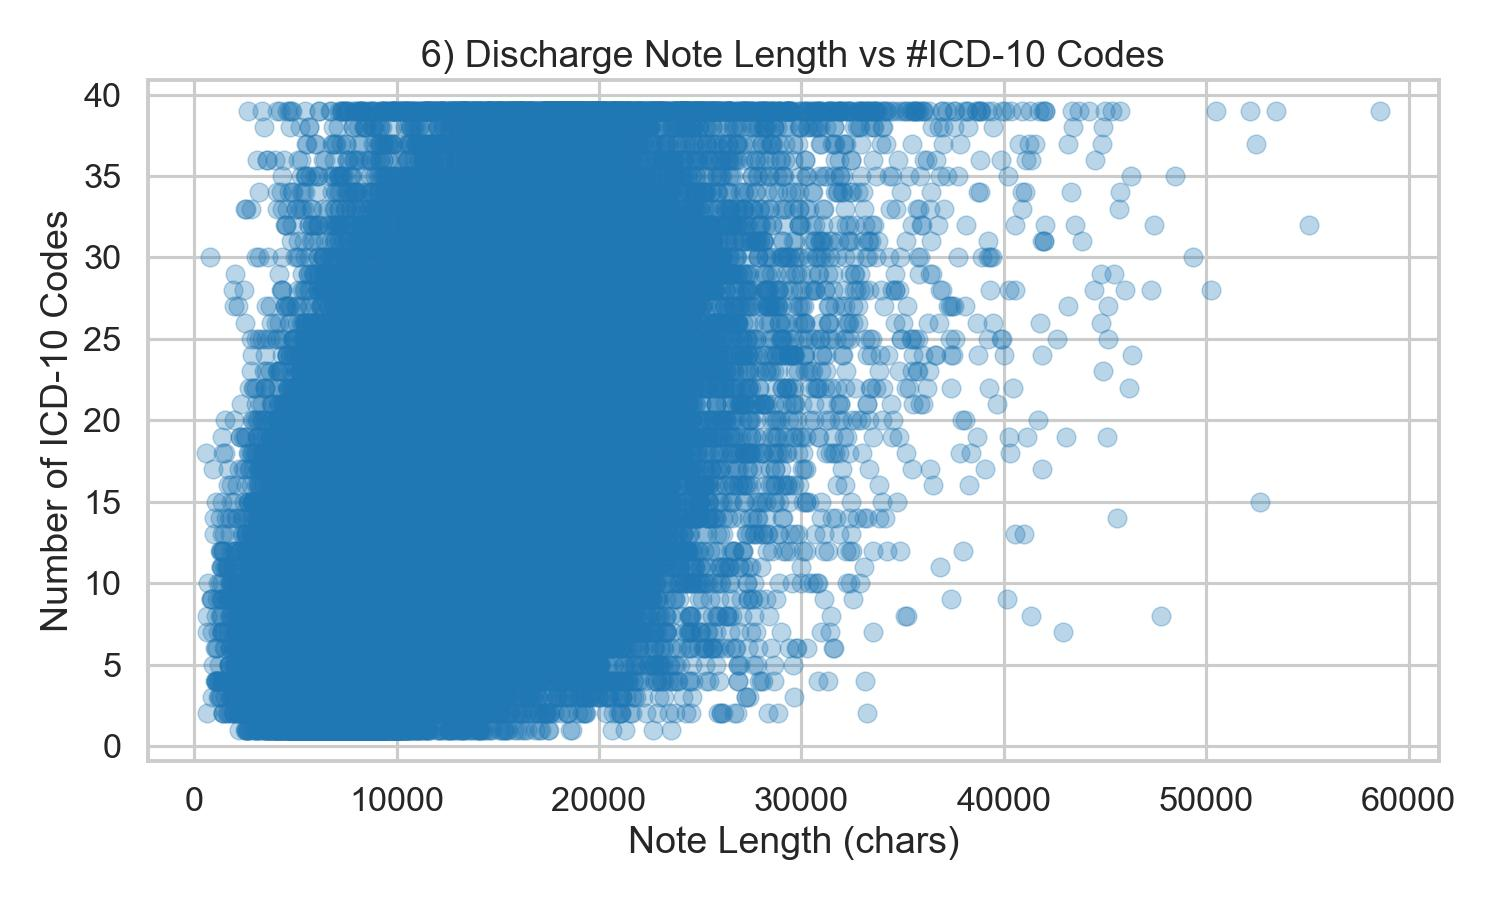
\includegraphics[width=0.5\textwidth]{mimic_plots/plot6.jpg}
    \caption{A scatter plot highlighting the relationship between note length (in characters) and the number of ICD-10 codes.}
    \label{fig:p1:plot6}
\end{figure}

\noindent
Figure~\ref{fig:p1:plot6} demonstrates a positive correlation: admissions with more diagnoses often generate longer discharge summaries. However, many cases are concentrated below 20,000 characters, indicating that moderately sized notes can still have multiple codes.

\newpage

\subsubsection*{Plot 7: Violin Plot of Code Counts by Anchor Year Group}
\begin{figure}[H]
    \centering
    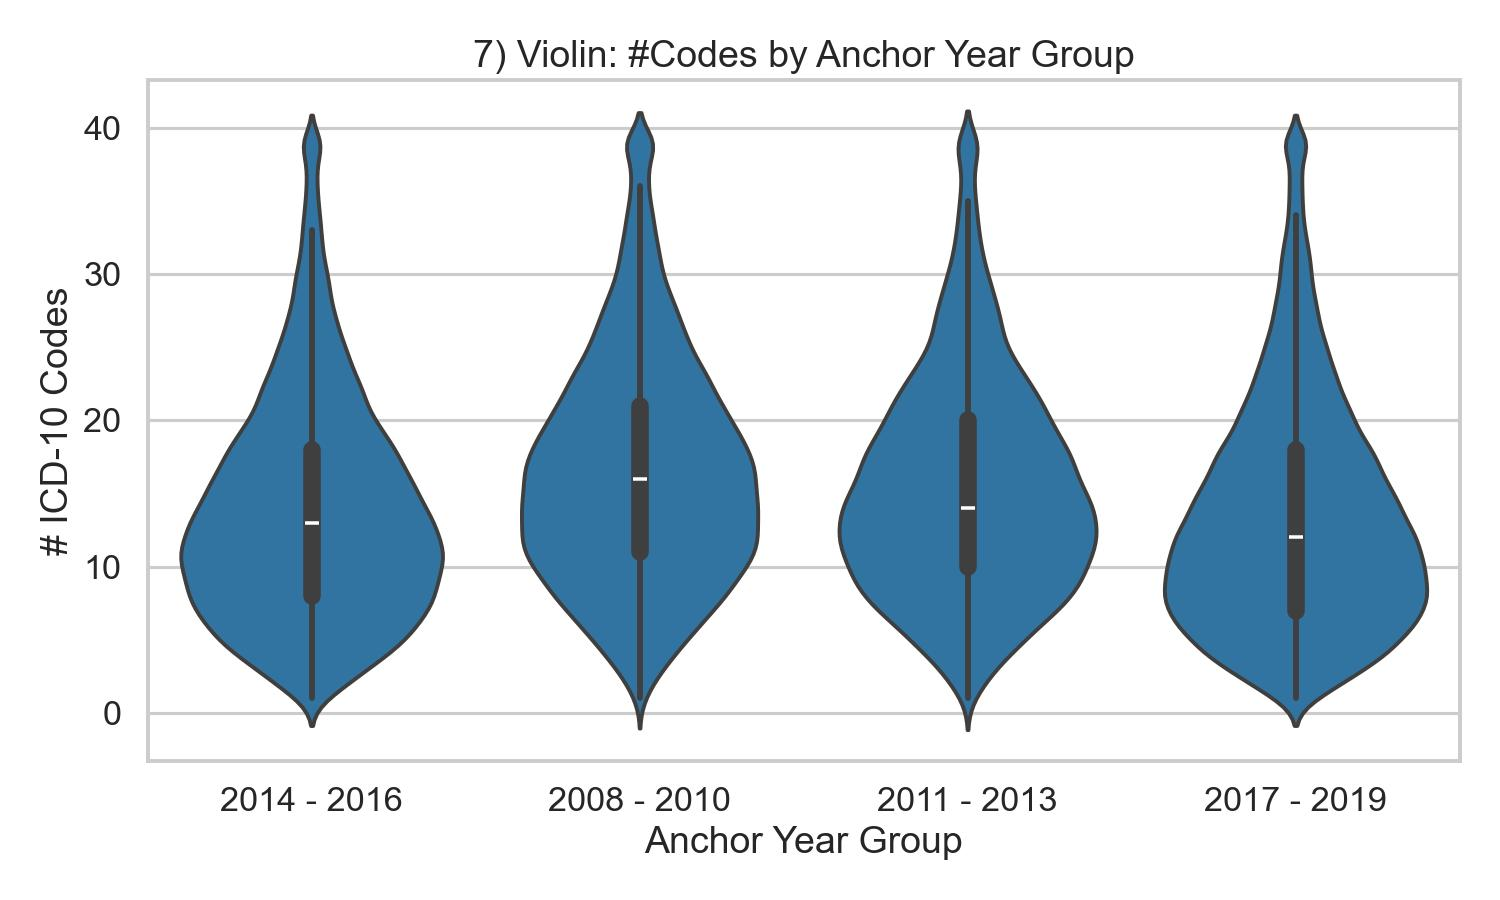
\includegraphics[width=0.5\textwidth]{mimic_plots/plot7.jpg}
    \caption{A violin plot representing how the distribution of total ICD-10 codes per admission varies across anchor year groups.}
    \label{fig:p1:plot7}
\end{figure}

\noindent
Figure~\ref{fig:p1:plot7} visualizes the spread of ICD-10 code counts for each time interval. Wide tails indicate that certain admissions receive a very large number of codes, reflecting complex clinical circumstances.

\newpage

\subsubsection*{Plot 8: Mean Discharge Note Length by Anchor Year Group}
\begin{figure}[H]
    \centering
    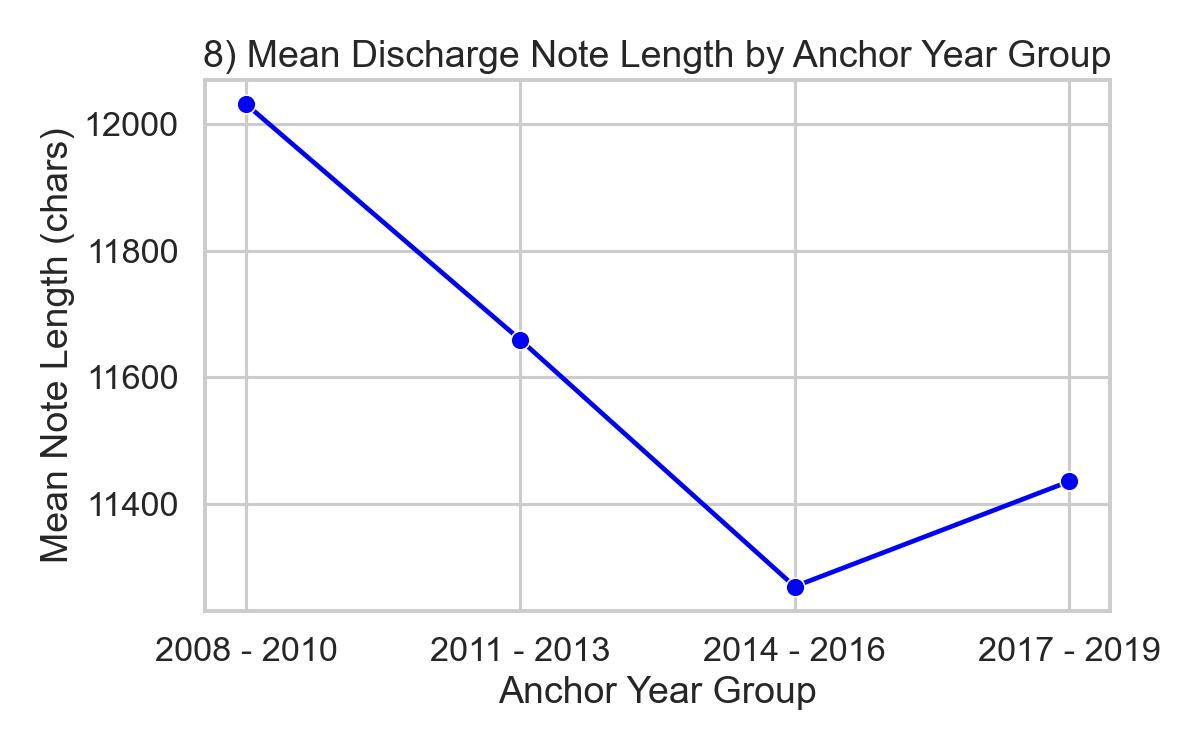
\includegraphics[width=0.5\textwidth]{mimic_plots/plot8.jpg}
    \caption{A line plot tracking average discharge summary lengths over five anchor year group intervals.}
    \label{fig:p1:plot8}
\end{figure}

\noindent
Figure~\ref{fig:p1:plot8} suggests that longer average notes were generated during the earlier collection periods (2008--2010), followed by a dip in 2014--2016 and a partial rebound in later intervals. Evolving clinical documentation practices may contribute to these shifts.

\newpage

\subsubsection*{Plot 9: Top 10 Admission Types by Volume}
\begin{figure}[H]
    \centering
    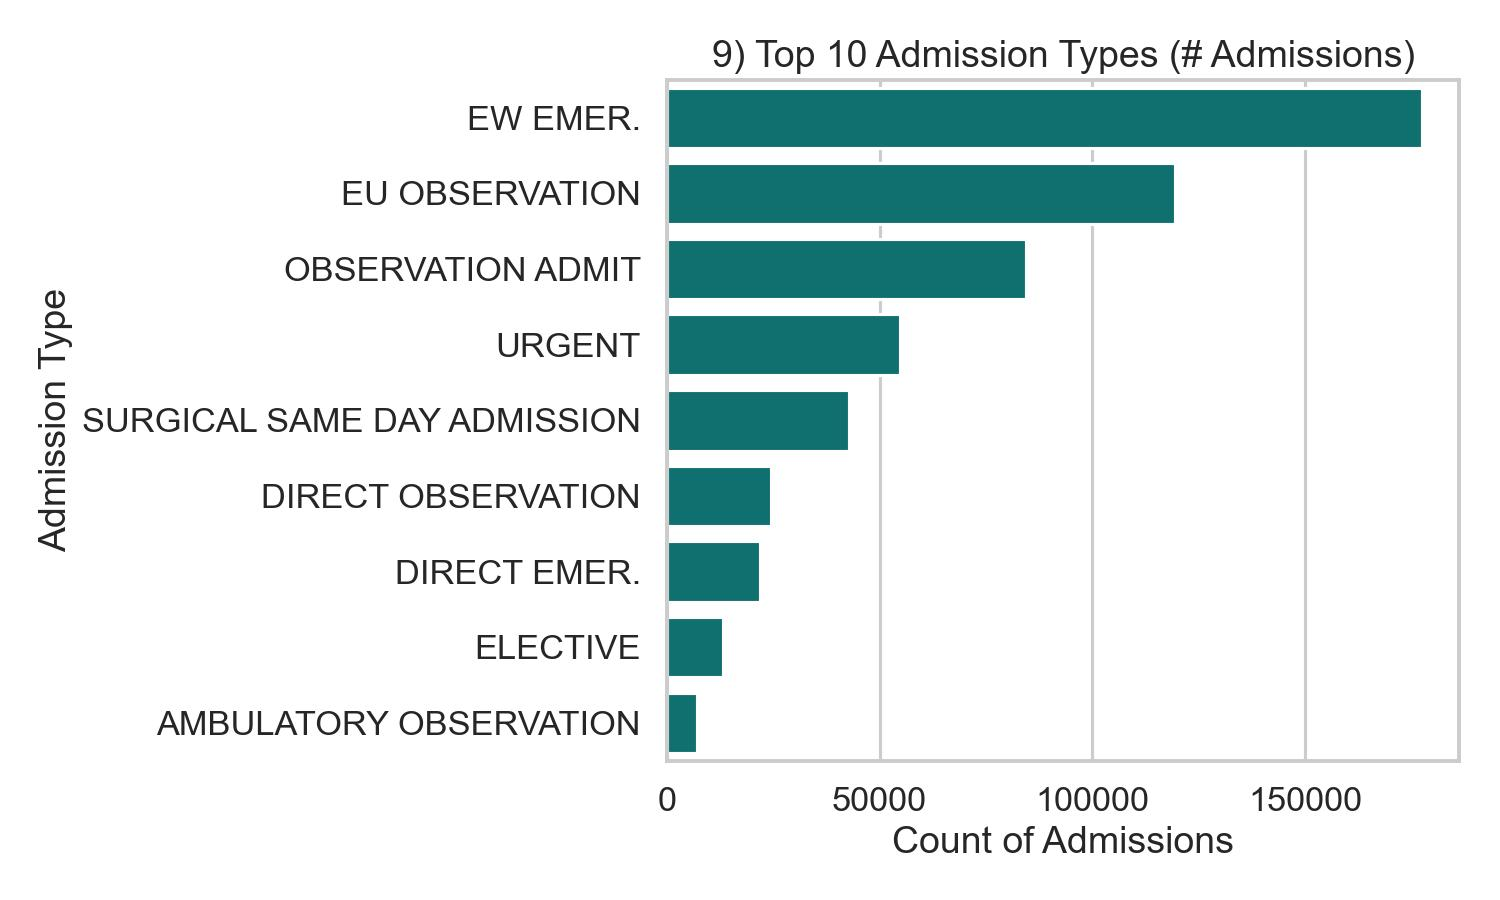
\includegraphics[width=0.5\textwidth]{mimic_plots/plot9.jpg}
    \caption{A horizontal bar chart showing the top ten admission types (e.g., emergency, elective, urgent).}
    \label{fig:p1:plot9}
\end{figure}

\noindent
Figure~\ref{fig:p1:plot9} highlights the prominence of emergency or unplanned admissions. Emergency admissions dominate, but there are also notable volumes in scheduled categories such as elective surgeries.

\newpage

\subsubsection*{Plot 10: ICD-10 Code Frequency by Anchor Year Group (Top 15 Codes)}
\begin{figure}[H]
    \centering
    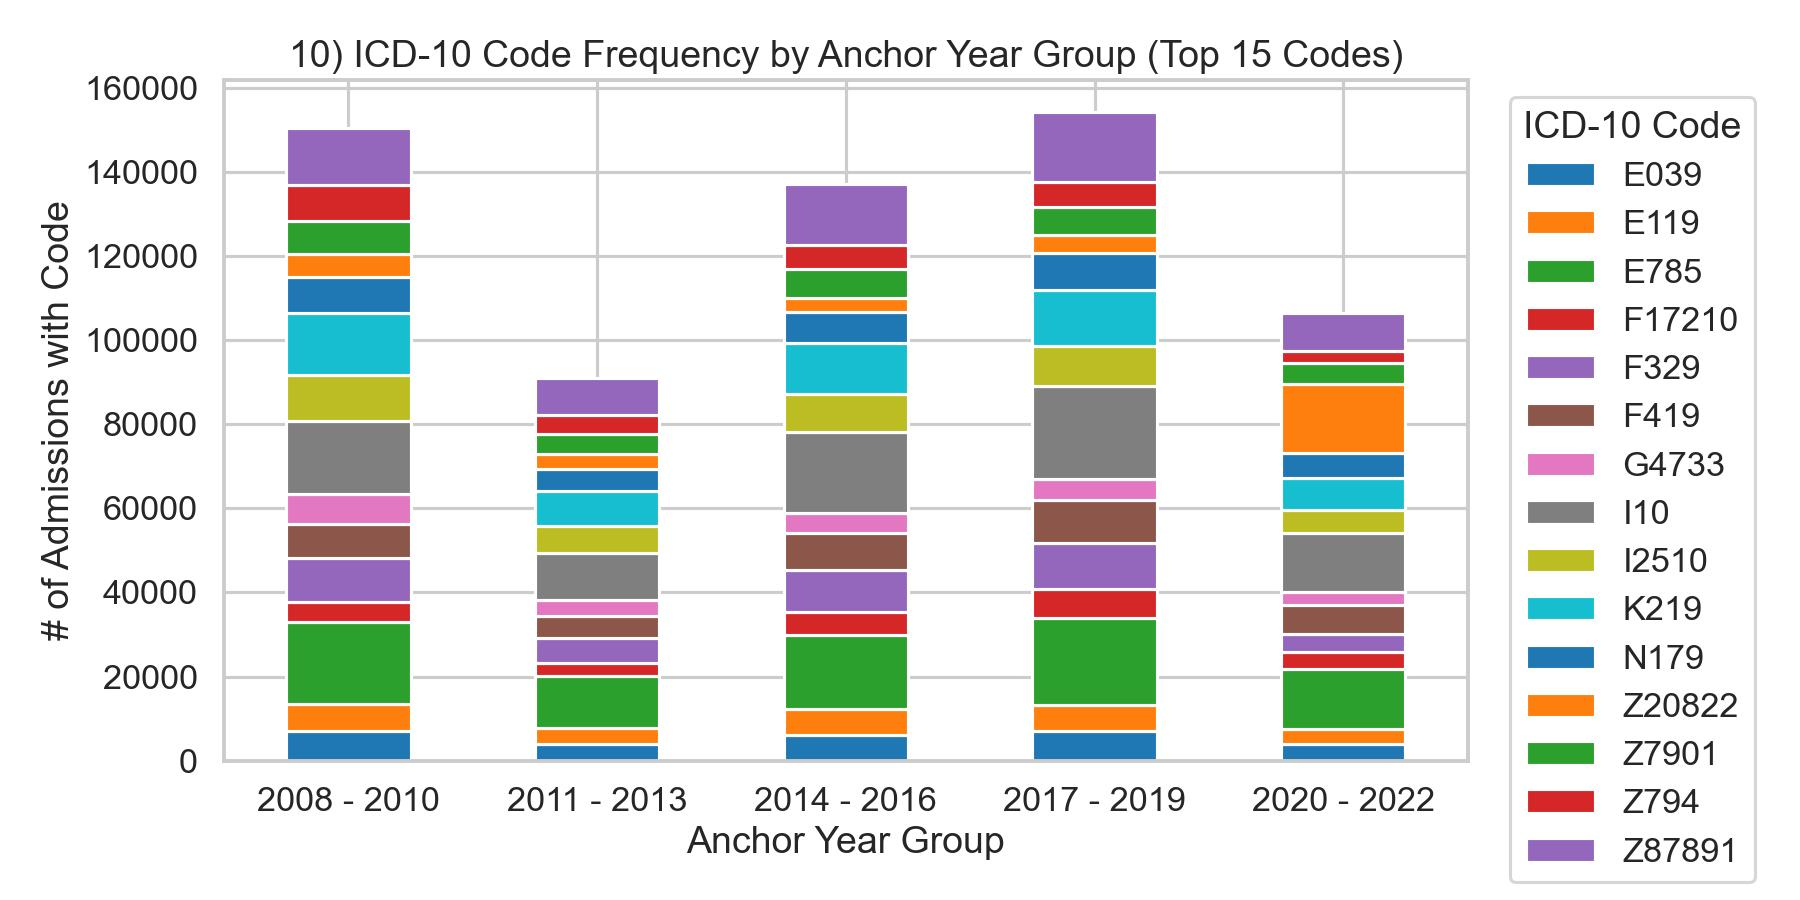
\includegraphics[width=0.5\textwidth]{mimic_plots/plot10.jpg}
    \caption{A stacked bar chart displaying the occurrence of each top-15 ICD-10 code within different anchor year groups.}
    \label{fig:p1:plot10}
\end{figure}

\noindent
Figure~\ref{fig:p1:plot10} shows that certain diagnoses remain consistently frequent across all anchor year intervals, again reflecting the prevalence of long-standing chronic conditions such as metabolic disorders and cardiovascular disease.

\subsection{Key Insights}\label{sec:p1:key_insights}
\noindent
From these queries and visualizations, several points emerge:
\begin{itemize}
    \item \textbf{Large-Scale Data:} There are more than 364k unique patients and over 546k admissions, providing robust coverage of a hospital population.
    \item \textbf{Multiple Diagnoses:} The average admission carries more than 13 ICD-10 codes, confirming a multi-label setting.
    \item \textbf{Long-Tail Challenge:} Over 9,217 ICD-10 codes appear fewer than five times, highlighting difficulties with rare or specialized diagnoses.
    \item \textbf{Varied Note Lengths:} Discharge summaries range from brief texts to lengthy narratives with thousands of words.
\end{itemize}

\subsection{Final Data Preparation}\label{sec:p1:final_data_preparation}
\noindent
For the goal of building a text-to-ICD coding model (akin to AWS Comprehend Medical or other automated medical coding applications), a consolidated table was created that merges each admission's discharge note with the set of associated ICD-10 codes. The approach takes each row in the \texttt{discharge} table, then joins it with the corresponding entries in \texttt{diagnoses\_icd} for that \texttt{hadm\_id}. 

\vspace{5pt}
\noindent
The final consolidated table was created by joining each admission's discharge note with the corresponding entries in \texttt{diagnoses\_icd} for that \texttt{hadm\_id}. Each row in the resulting table contains:
\begin{itemize}
    \item \textbf{notes}: The original discharge summary (raw text).
    \item \textbf{icd\_codes}: A comma-separated list of all ICD-10 codes assigned to that admission.
\end{itemize}

\vspace{5pt}
\noindent
This design directly supports multi-label classification, as the full narrative of the discharge summary is provided (with no additional demographic or structural metadata) alongside all billed ICD-10 codes. Such a format simulates real-world scenarios in which only free-text documentation is available for downstream coding or NLP tasks.

%% ================================================================
%%  PART II — SA-AKI Cohort (Problem 2)  [Current Report — VERBATIM]
%% ================================================================
\section{Part II: SA-AKI Cohort (Problem 2)}\label{sec:p2:dataset}

\subsection{Overview}
The data assets and clinical labeling rules that underlie the analysis-ready SA--AKI cohort are described first, followed by the temporal conventions and harmonization steps that precede the main analysis. The remainder of the chapter is devoted to the Exploratory Data Analysis (EDA) conducted on the training set. That EDA serves as a form of unsupervised phenotyping: it identifies the clinical characteristics and risk factors that differentiate patient outcomes and provides the empirical foundation for the predictive modeling that follows.

\subsection{Source Tables and Warehouse Context}
Figure~\ref{fig:data-universe} positions the raw inputs within MIMIC--IV (core, hosp, ICU) that were ingested and optimized in the warehouse. These tables provide the vitals, labs, medications, microbiology, and encounter scaffolding used for labeling and features.

\begin{figure}[htbp]
    \centering
    \makebox[\linewidth][c]{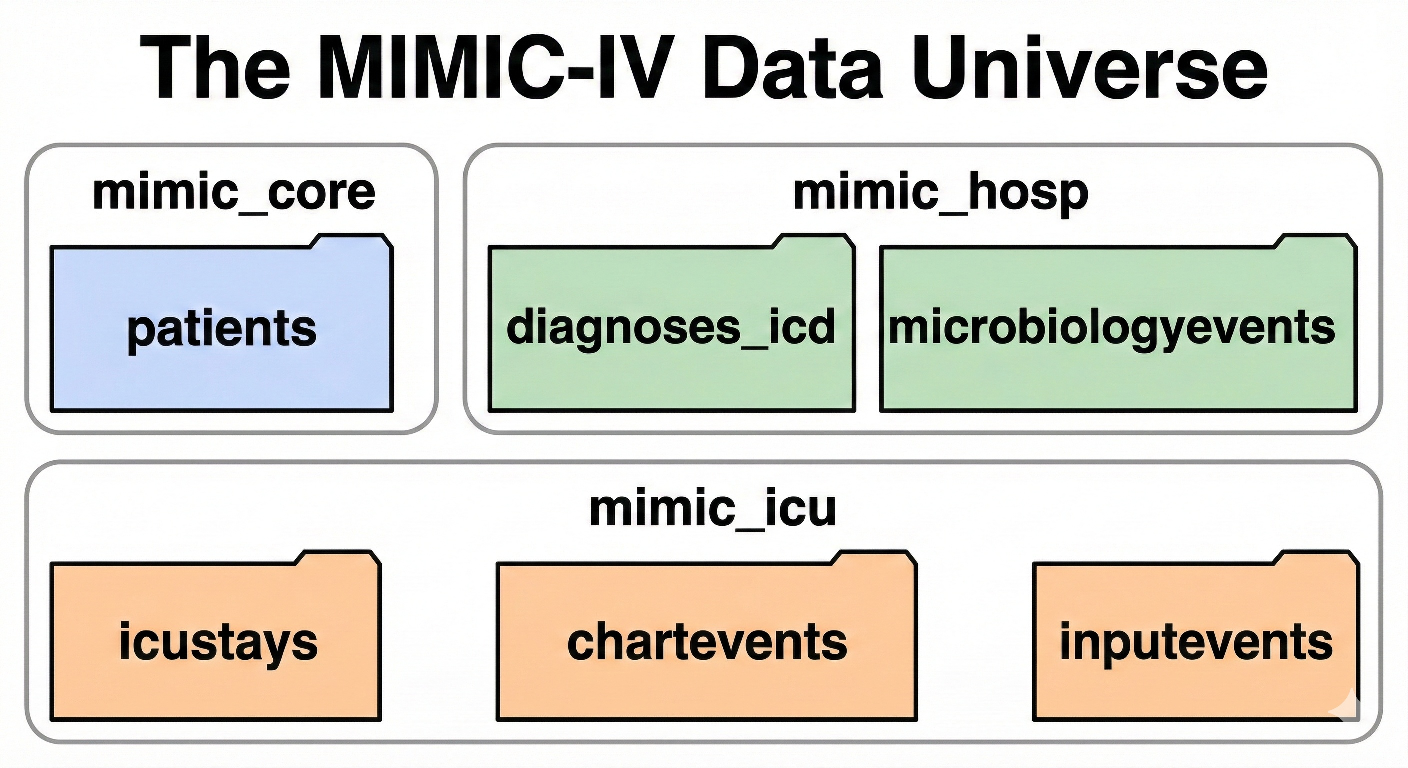
\includegraphics[width=\linewidth]{dataset_images/1_data_universe.pdf}}
    \caption{MIMIC--IV data universe leveraged in this study.}
    \label{fig:data-universe}
\end{figure}

\subsection{Ontology-Driven Concept Identification}
To avoid brittle, hard-coded drug lists, clinical concepts were mapped across terminologies and ingredient-level value sets were derived programmatically. The crosswalk in Figure~\ref{fig:ontology-crosswalk} illustrates the pathway from SNOMED~CT through UMLS CUIs into RxNorm ingredients, with ATC used as an orthogonal cross-reference and coverage check. This pipeline underlies the systemic \emph{antibiotic} and \emph{vasopressor} flags used in labeling and feature construction.

\begin{figure}[htbp]
    \centering
    \makebox[\linewidth][c]{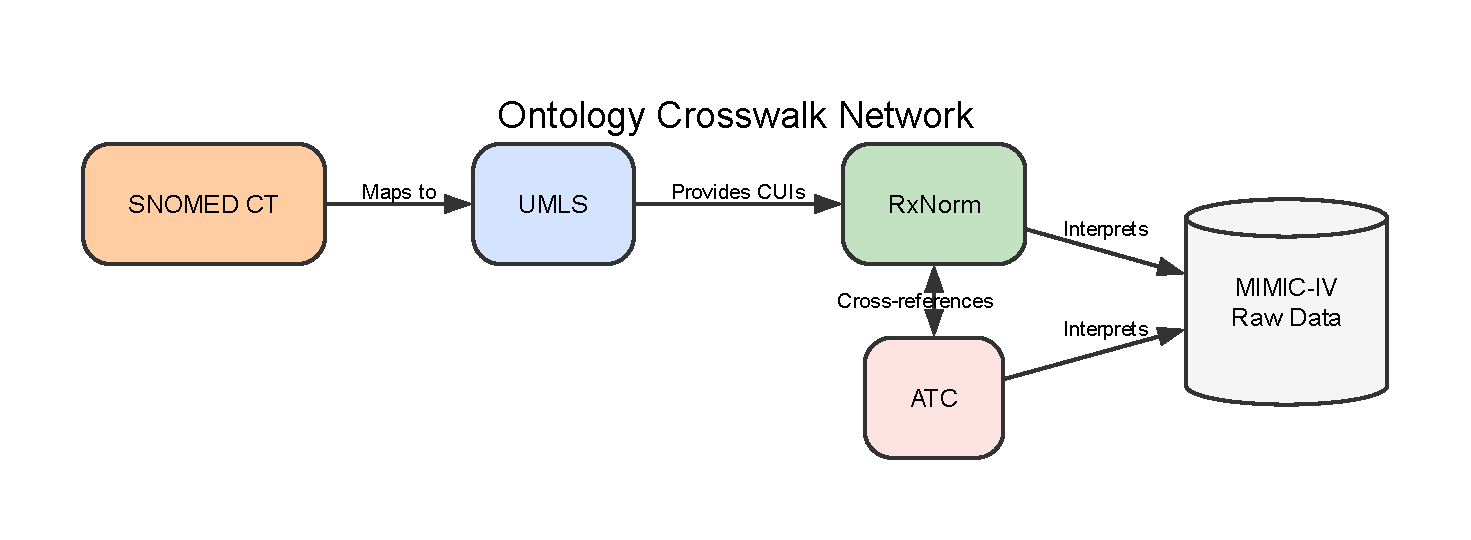
\includegraphics[width=\linewidth]{dataset_images/7_ontology_crosswalk}}
    \caption{Ontology crosswalk linking SNOMED~CT $\rightarrow$ UMLS CUIs $\rightarrow$ RxNorm ingredients, with ATC cross-reference.}
    \label{fig:ontology-crosswalk}
\end{figure}

\subsection{Cohort Construction (Counts and Exclusions)}
A CONSORT-style reduction from all ICU stays to the final analysis cohort was followed. Figure~\ref{fig:consort} consolidates inclusion criteria (adult, first ICU stay, LOS~$\ge$~24\,h), Sepsis--3 screening, SA--AKI temporal linkage, and final exclusions (ESRD, early RRT). These counts serve as the reference for all summary denominators used in the EDA.

\begin{figure}[htbp]
    \centering
    \makebox[\linewidth][c]{
\includegraphics[width=\linewidth]{dataset_images/8_consort_flow}}
    \caption{CONSORT-style flow of cohort construction with key exclusions.}
    \label{fig:consort}
\end{figure}

\subsection{Clinical Labeling Rules and Time Anchors}
\subsubsection{Sepsis--3 and AKI Logic (Compact View)}
Sepsis--3 requires \emph{suspected infection} \emph{and} an acute increase in organ dysfunction ($\Delta$SOFA~$\ge$~2). AKI follows KDIGO using three criteria: serum creatinine (absolute/relative) and urine output (UO). The Sepsis--3 gate and the UO sessionization used for the KDIGO UO criterion are displayed as a two-panel composite in Figure~\ref{fig:logic-composite}.

\begin{figure}[htbp]
    \centering
    \begin{subfigure}{0.48\linewidth}
        \centering
        
\includegraphics[width=\linewidth]{dataset_images/10_sepsis3_and_logic}
        \caption{Sepsis--3 core logic gate.}
    \end{subfigure}\hfill
    \begin{subfigure}{0.48\linewidth}
        \centering
        
\includegraphics[width=\linewidth]{dataset_images/9_urine_output_logic}
        \caption{UO sessionization for KDIGO (continuous windows $<$0.5\,mL/kg/h for $\ge$6\,h).}
    \end{subfigure}
    \caption{Clinical rule components used for cohort labeling.}
    \label{fig:logic-composite}
\end{figure}

\subsubsection{Timeline Conventions and Windows}
All predictors used in modeling are restricted to the first 24\,h after ICU admission (T0--T24). Suspected infection is defined by a temporal link between cultures and systemic antibiotics, and SA--AKI requires AKI onset within $\pm$48\,h of Sepsis onset. Figure~\ref{fig:timeline} illustrates these anchors and windows.

\begin{figure}[htbp]
    \centering
    \makebox[\linewidth][c]{
\includegraphics[width=\linewidth]{dataset_images/6_final_timeline}}
    \caption{Illustrative patient journey with T0--T24 feature window, infection window, Sepsis onset, and AKI onset; the SA--AKI link is $\pm$48\,h around Sepsis onset.}
    \label{fig:timeline}
\end{figure}

\subsection{Data Harmonization and Initial Statistics}
Before any analysis, data were harmonized (e.g., Fahrenheit~$\rightarrow$~Celsius), redundant features were removed, and comorbidities were consolidated. The final analytic cohort contained \textbf{n=10,036} ICU stays. A stratified 80/20 split resulted in a training set of 8,028 patients and a test set of 2,008 patients. The in-hospital mortality rate in the training set was 26.74\%. Key baseline statistics are presented in Table~\ref{tab:snapshot} and Table~\ref{tab:therapies-prev}.

\begin{table}[htb!]
    \centering
    \caption{Overall cohort snapshot (final build).}
    \label{tab:snapshot}
    \small
    \begin{tabular}{ll}
        \toprule
        \textbf{Metric} & \textbf{Value}\\
        \midrule
        In-hospital death & \textbf{26.7\%} (2,684/10,036)\\
        Male & \textbf{53.0\%} (5,322/10,036)\\
        AKI trigger = Creatinine (vs.\ Urine Output) & \textbf{40.7\%} (4,087/10,036)\\
        \bottomrule
    \end{tabular}
\end{table}

\begin{table}[htb!]
    \centering
    \caption{Therapy/exposure prevalence in the first 24\,h (1/0 encoding).}
    \label{tab:therapies-prev}
    \small
    \begin{tabular}{ll}
        \toprule
        \textbf{Day-1 therapy / exposure flag} & \textbf{Prevalence} \\
        \midrule
        Mechanical ventilation within 24\,h & \textbf{53.0\%} (5,320/10,036) \\
        Vasopressor within 24\,h & \textbf{36.6\%} (3,676/10,036) \\
        Renal replacement therapy within 24\,h & \textbf{69.0\%} (6,922/10,036) \\
        \bottomrule
    \end{tabular}
\end{table}

\subsection{Exploratory Analysis and Phenotyping of the Training Cohort}

\subsubsection{Statistical Validation of Data Integrity}
A foundational step of the EDA was to statistically validate the cohort and the train-test split. As shown in Figure~\ref{fig:statistical_testing_eda}, key clinical variables exhibited highly significant differences between survivor and non-survivor groups within the training set (all $p < 0.001$, Mann-Whitney U test), suggesting that the selected features contain a strong prognostic signal. The same tests revealed no significant distributional differences for these variables between the training and test sets (all $p > 0.05$), indicating that the stratified split was successful and that the test set may be regarded as a representative sample for evaluating final model performance.

\begin{figure}[htb!]
    \centering
    \makebox[\textwidth][c]{
\includegraphics[width=\textwidth]{preprocessing_images/statistical_testing.png}}
    \caption{Statistical significance of key clinical variables between survivor and non-survivor groups, confirming that the selected features carry a strong prognostic signal ($p < 0.001$, Mann-Whitney U test).}
    \label{fig:statistical_testing_eda}
\end{figure}

\subsubsection{Analysis of Missing Data Patterns}
The pattern of missing data was investigated as a potential source of information. Of the 161 initial features, 101 had missing values. Little's MCAR test strongly rejected the null hypothesis ($p \approx 0.0$), indicating the data were not Missing Completely At Random. A subsequent chi-square analysis revealed that the absence of 46 specific measurements was significantly associated with mortality ($p < 0.05$). The ten most significant associations are shown in Table~\ref{tab:missingness_assoc_eda}, highlighting that the absence of liver function and tissue injury tests was highly prognostic. These findings suggest that patterns of clinical data collection are themselves informative predictors of outcome.

\begin{table}[htb!]
    \centering
    \caption{Top 10 most significant associations between missingness indicators and in-hospital mortality.}
    \label{tab:missingness_assoc_eda}
    \small
    \begin{tabular}{lrrr}
        \toprule
        \textbf{Indicator} & \textbf{Chi-Square} & \textbf{p-value} & \textbf{Cramér's V} \\
        \midrule
        \texttt{ast\_n\_missing} & 166.46 & $<0.001$ & 0.144 \\
        \texttt{ast\_max\_missing} & 166.46 & $<0.001$ & 0.144 \\
        \texttt{alkphos\_median\_missing} & 165.27 & $<0.001$ & 0.143 \\
        \texttt{alkphos\_n\_missing} & 165.27 & $<0.001$ & 0.143 \\
        \texttt{tbili\_n\_missing} & 163.90 & $<0.001$ & 0.143 \\
        \texttt{tbili\_max\_mgdl\_missing} & 163.90 & $<0.001$ & 0.143 \\
        \texttt{ldh\_max\_ul\_missing} & 96.66 & $<0.001$ & 0.110 \\
        \texttt{ldh\_n\_missing} & 96.66 & $<0.001$ & 0.110 \\
        \texttt{calcium\_n\_missing} & 73.11 & $<0.001$ & 0.095 \\
        \texttt{calcium\_min\_missing} & 73.11 & $<0.001$ & 0.095 \\
        \bottomrule
    \end{tabular}
\end{table}

\subsubsection{Clinical Phenotypes of Survivor vs. Non-Survivor Groups}
The EDA revealed distinct clinical phenotypes between survivors and non-survivors in the training set. As illustrated in Figure~\ref{fig:eda_distributions_eda}, non-survivors were significantly older and had higher baseline severity of illness, reflected by higher APACHE~III and SOFA scores. Physiologically, the non-survivor phenotype was characterized by more severe multi-organ dysfunction, including worse renal function (higher maximum creatinine) and greater metabolic distress (higher maximum lactate).

\begin{figure}[htb!]
    \centering
    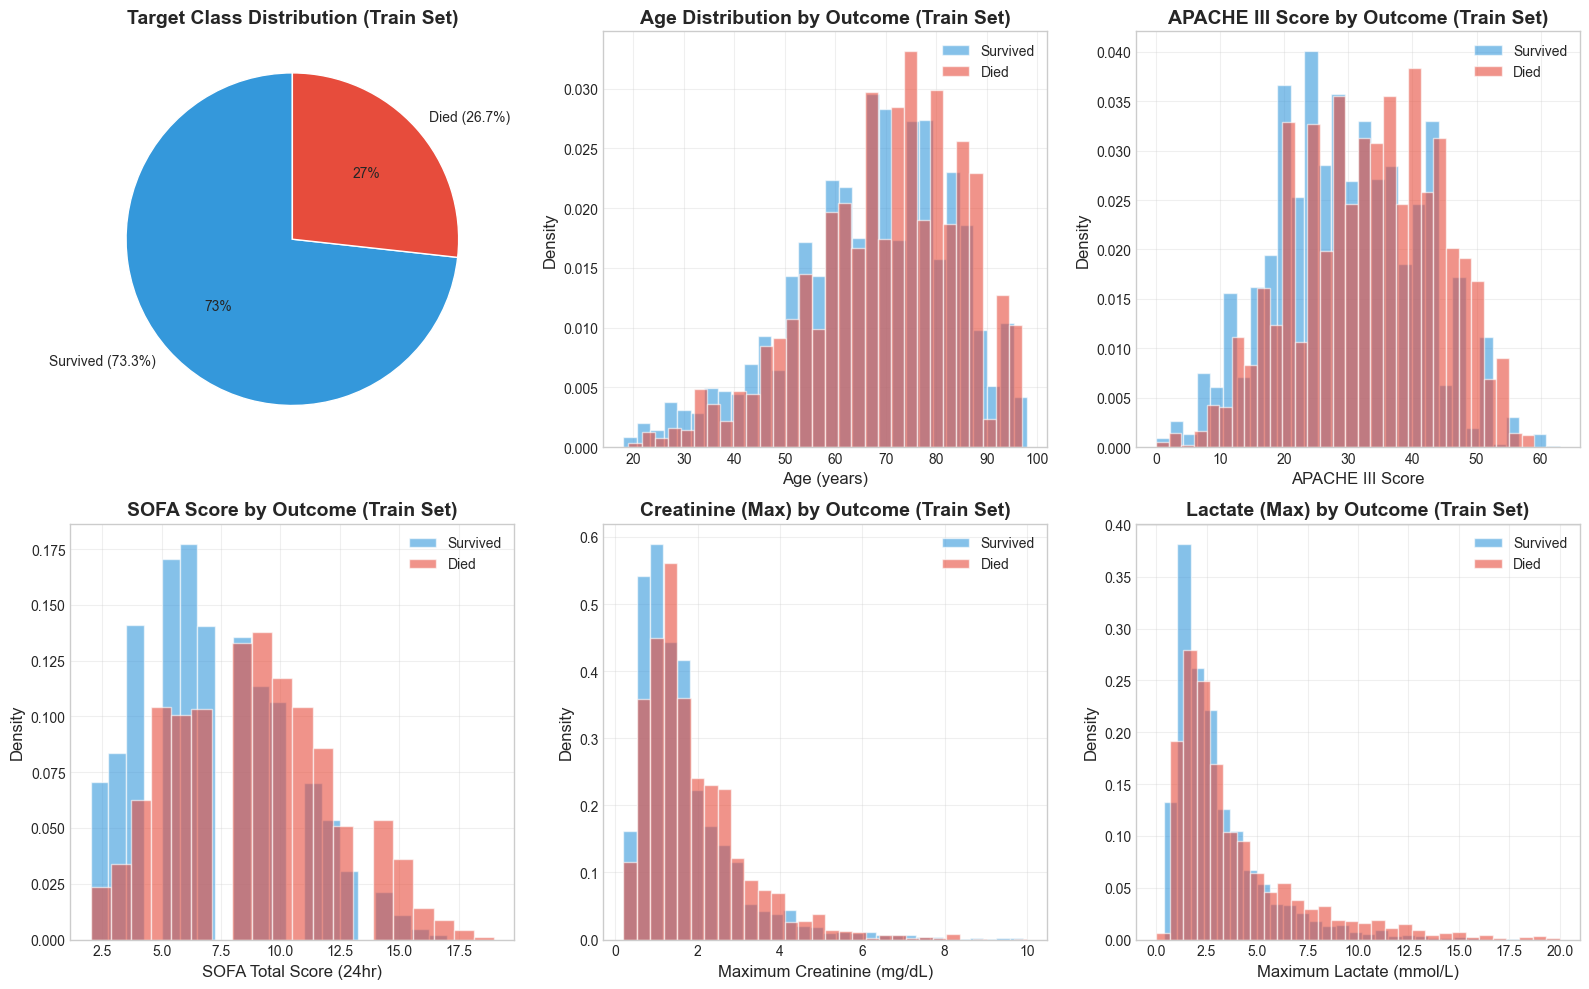
\includegraphics[width=\textwidth]{preprocessing_images/eda_distributions.png}
    \caption{Distributions of key clinical variables in the training set, stratified by mortality outcome. Non-survivors consistently show distributions shifted towards higher severity.}
    \label{fig:eda_distributions_eda}
\end{figure}

This phenotyping was further supported by correlation analysis (Figure~\ref{fig:feature_correlations_eda}). The overall SOFA score (\texttt{sofa\_total\_24hr}) had the strongest positive correlation with death (0.234), reinforcing its role as a global marker of risk. Other features strongly associated with mortality included markers of hematological dysfunction (\texttt{rdw\_median\_pct}, 0.188) and hepatic injury (\texttt{sofa\_hepatic\_24hr}, 0.169). In contrast, variables indicating physiological stability and adequate organ perfusion, such as total urine output (\texttt{urine\_output\_total\_24hr}, -0.113) and minimum pH (\texttt{ph\_min}, -0.101), were the strongest predictors of survival. Together, these findings provide a data-driven characterization of the high-risk SA--AKI patient and directly informed the feature set for supervised modeling.

\begin{figure}[htb!]
    \centering
    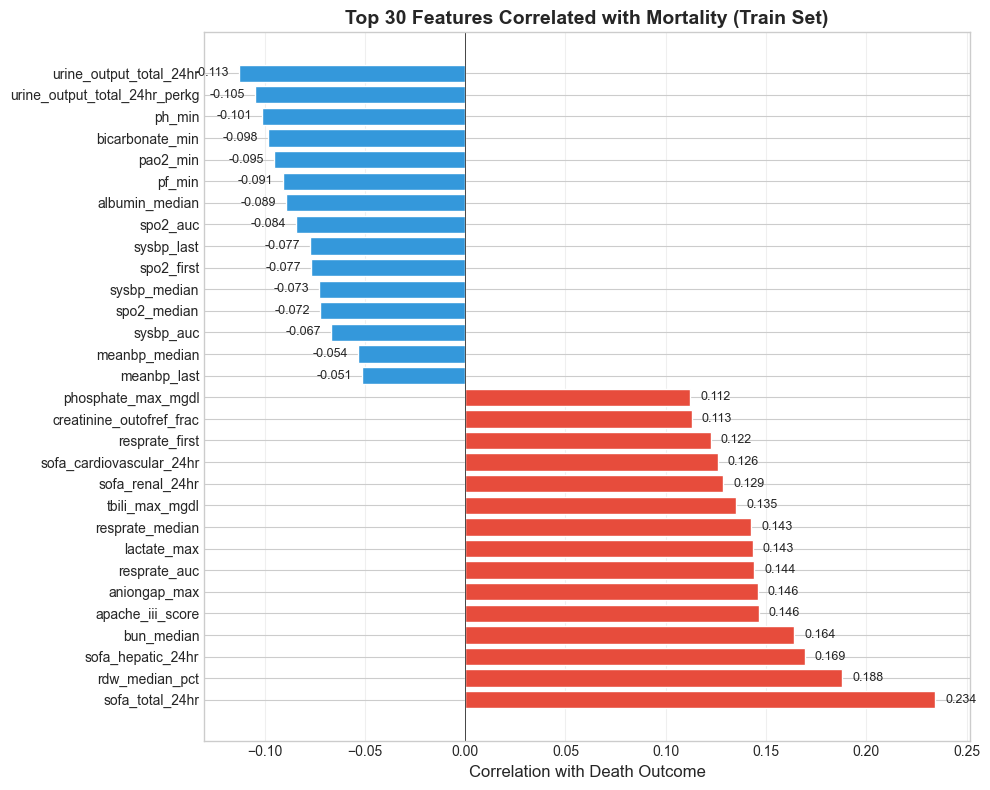
\includegraphics[width=0.8\textwidth]{preprocessing_images/feature_correlations.png}
    \caption{Top 30 features with the strongest positive (red) and negative (blue) correlation with in-hospital mortality in the training set.}
    \label{fig:feature_correlations_eda}
\end{figure}
